\documentclass[12pt]{article}
\usepackage[margin=0.9in]{geometry} 
\usepackage[utf8]{inputenc}
\usepackage{amsmath}
\usepackage{amsfonts}
\usepackage{amssymb}
\usepackage{graphicx}
\usepackage{color}
\usepackage{float}
\usepackage{scrextend}
\usepackage{enumitem}
\usepackage{parskip}
\usepackage{siunitx}
%\usepackage{listings}

%ignore \hbox issue
\hfuzz=100pt


% title declarations
\newcommand{\doctitle}{Project 3 - The MOS Transistor}
\newcommand{\docsubtitle}{Noise Margins, VTC and Cadence Simulations}

\renewcommand{\maketitle} {
    \setlength{\parindent}{0pt}
    \begin{center} \
        % top spacing
        \vspace*{1in}

        % main title
        \huge{\doctitle}\\
        \Large{\docsubtitle}

        % naming
        \vspace*{0.2in}
        \large{
            Arthur Hsueh\\
            21582168\\
            UBC - ELEC 402
        }
    \end{center}
}

\begin{document}
\maketitle
\thispagestyle{empty}
\pagebreak

\tableofcontents
\thispagestyle{empty}
\pagebreak

\listoffigures
\thispagestyle{empty}

\listoftables
\thispagestyle{empty}

\pagebreak
\setcounter{page}{1}

\section{Designing widths of pull-down transistors}
This problem asks to design the widths of the pull-down transistors such that $V_{OL}$ = 0.1 V. The general
method is to equate $I_{L}$, the current from the load resistor/transsitor, to $I_{DI}$, the drain current of the 
pull-down transistor. Because we are evalulating for the design requirement of $V_{OL}$, we take the input as
$V_{in} = V_{DD}$, and thus the pull-down transistor will always be in the linear regime.
\subsection{Calculations}

\subsection*{Resistive load inverter}
This is the circuit that contains the 10k$\Omega$ resistor. We begin by equating currents,
\[ I_R = I_{D}(linear) \]
\[\frac{V_{DD} - V_{OL}}{R_L} = \frac{W_N}{L_N} \mu_N C_{ox} ((V_{DD} - V_T) V_{OL} - \frac{V_{OL}^2}{2}) \]
Values can be substituted in, (constants used will be taken from the Useful\_Formula.pdf document on canvas)
\[\frac{1.2 - 0.1}{10000} = \frac{W_N}{0.1*10^{-7}}*270*1.6*10^{-6} *((1.2 - 0.4)*0.1 - \frac{0.1^2}{2}) \]
Solving for $W_N$ yields
\[ W_N = 3.395 * 10^{-8}m = 33.95 nm\]

\subsection*{Saturated-enhancement-load inverter}
This is the circuit that contains the pull-up NMOS transistor with 1.2V gate voltage. Here, the pull-up
transistor is operating in the satuation regime ($V_{DS} > V_{GS} - V_T$). Again, we equate curents to solve,
\[ I_{S pull-up}(saturation) = I_{D}(linear)\]
\[\frac{W_L v_{sat}C_{ox}(V_{DD} - V_{OL} - V_{TL})^2}{(V_{DD} - V_{OL} - V_{TL}) + E_C L_L} = \frac{W_N}{L_N} \mu_N C_{ox} ((V_{DD} - V_T)V_{OL} - \frac{V_{OL}^2}{2}) \]
Substituting values,
\[\frac{0.1*10^{-5}* 8*10^6 *1.6 * 10^{-6}(1.2 - 0.1 - 0.4)^2}{(1.2 - 0.1 - 0.4) + 6*0.1*10^{-7}} = \frac{W_N}{0.1*10^{-7}}*270*1.6*10^{-6} *((1.2 - 0.4)*0.1 - \frac{0.1^2}{2})\]
Solving for $W_N$ yields
\[ W_N = 2.765*10^-9m = 2.765nm\]

\subsection*{'Linear'-load inverter}
This is the circuit that contains the pull-up NMOS transistor with 1.6V gate voltage. Here, the pull-up transistor
is operating in the linear regime ($V_{DS} < V_{GS} - V_T$). This calculation allows for cancellation of many terms
Again, we equate currents to solve,
\[ I_{S pull-up}(linear) = I_{D}(linear)\]
Cancelling identical terms yields,
\[W_L ((V_{gate} - V_{OL} - V_T) V_{OL} - \frac{V_{OL}^2}{2}) = W_N ((V_{DD} - V_T) V_{OL} - \frac{V_{OL}^2}{2}) \]
Substituting values,
\[0.1*10^{-7} ((1.6 - 0.1 - 0.4)*0.1 - \frac{0.1^2}{2}) = W_N ((1.2 - 0.4)*0.1 - \frac{0.1^2}{2}) \]
Solving for $W_N$ yields 
\[ W_N = 1.4*10^{-8} = 14nm\]

\subsection{Results}
The calculated values of $W_N$ are reiterated below, with all values with units of nm.
\begin{table} [H]
    \centering
    \begin{tabular} {ccc} 
        Resistive & Saturated-enhancement & 'Linear'\\
        \hline
        33.95 & 2.765 & 14
    \end{tabular}
    \caption{Calculated widths for each of the 3 inverters}
\end{table}
We notice that the resistive load inverter requires the largest width, followed by the 'linear' inverter and then the saturated-enhancement inverter. 

When we
design for $V_{OL}$ we treating the inverter as if it has been inputted logic high and outputs logic low. So, the pull-down transistor is always in the linear 
region and can be modelled as a small resistor. So, ideally we want the pull-up network to be comparatively much larger in resistance (voltage divider property
applies here). In an ideal inverter, we would experience infinite resistance in the pull-up network, and zero resistance in the pull-down network.

If we look at the saturated-enhancement-load inverter, the pull-up NMOS transistor is operating in the saturation region which can be modelled as
a current source. The closer we are to an ideal current source, $V_{DS} << V_{GS} - V_T$ the closer we are to an infinite resistance. For the 'linear'-load inverter
the pull-up NMOS is operating exactly on the boundary between linear and saturation.

The effective resistance of the pull-up network will directly affect the width of the pull-down network transistors. 
We want to adjust the pull-down transistor to match the effective resistance of the pull-up network for a low $V_{OL}$. A high $W_N$ value means a low resistance,
and a low $W_N$ value means a high resistance. The calculated values reflect the relative offset of this property. The saturated inverter needs a high resistance
to balance for $V_OL$, the 'linear' inverter need a slightly lower resistance to balance, and the resistive load inverter has a large resistor to pull-up, so it 
doesnt need as big of a resistance to pull-down.


\pagebreak

\section{Determining purpose and VTC of unknown circuit}
\subsection{Circuit Function and Output Swing}
The circuit visually resembles a CMOS inverter, but upon further inspection, the position of the PMSO and NMOS transistors are flipped.
The output is now at the source of both transistors. Looking at the truth table of the circuit, we can see the circuit appears to output the same
logic values as inputted.
\begin{table} [H]
    \centering
    \begin{tabular} {c|c}
        Logic IN & Logic OUT \\
        \hline
        0 & 0\\
        1 & 1\\
    \end{tabular}
    \caption{Logic table of the unknown circuit}
\end{table}
So, the circuit functions as a buffer. Thus, the output swings from a valid low to a valid low, and valid high to a valid high. 
Upon examination at the voltage level we notice that there are some differences, which will be discussed when
the voltage transfer characteristics are plotted in the next section.

\subsection{Plotting the VTC}
For an input of logic 1, $V_{in}$ = $V_{DD}$ = $V_{GS}$, the pull-up NMOS transistor operates in the saturation region, and the pull-down PMOS is off.
Here, the output is taken at the source terminals of the transistors. If we take into account the threshold voltage $V_T$ then we can say the \textbf{highest}
possible output voltage of this gate will always be $V_{DD} - V_T$. 

Likewise, for an input logic 0, $V_{in}$ = 0(theoretically) = $V_{GD}$, the pull down PMOS transistor operates in the saturation region. 
Again, taking into account the threshold voltage $V_T$ we can say the \textbf{lowest} possible output voltage of this gate will always be $V_T$.

Thus we have the values for $V_{OL}$ and $V_{OH}$
\[V_{OL} = \quad and \quad V_{OH} = V_{DD} - V_T\]

Below is a general plot of the VTC for the circuit.
\begin{figure} [H]
    \centering
    \makebox[\textwidth]{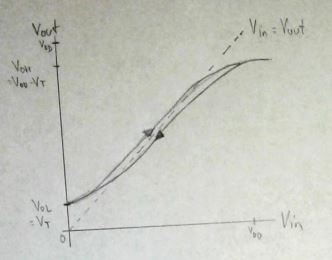
\includegraphics[scale=0.73]{../images/q2b_vtc.JPG}}
    \caption{The VTC of the unknown circuit}
\end {figure}
As the problem states, there is hysteresis in the VTC, because with the way the circuit is set up, when the input is $V_{OL}$ or $V_{OH}$ the output
will jump back to a linear operating regime. Looking at the line $V_{in} = V_{out}$, we can see that it intersect the VTC curve at two points, and
thus we have two switching voltages. For an input of $V_{OL}$, the output is expected to be 0 ($V_T$ in reality), and $V_{SD}$ becomes small, which
pushing the PMOS back into the linear regime. And likewise for an input of $V_{OH}$, the output is expected to be $V_{DD}$, ($V_{DD}$ - $V_T$ in reality),
and thus $V_{DS}$ become small, which pushes the NMOS back into the linear regime.
\subsection{Gain and Validity of the Circuit}
From the VTC plot, we can see that the circuit is not a valid gate. At the low gain areas of the VTC, near the levels of $V_{OL}$ and $V_{OH}$, it
is clear that the gain/slope at those areas are greater than one, which is not what we want. The high gain areas do satisfy a valid gate, but the
low gain areas don't. Because of the fact the low gain areas have slopes greater than one, this means that noise is not attenuated, rather amplified.

Another reason this circuit would not function well as a valid gate is because the output voltage level is now narrower, between $V_T$ and $V_{DD} - V_T$. 
The output will be fed as input to other gates, which ideally would still prefer input ranges of $V_{DD}$ and 0. 
\subsection{Validation using CAD Tools}
Below is the schematic that describes the circuit defined in the problem
\begin{figure} [H]
    \centering
    \makebox[\textwidth]{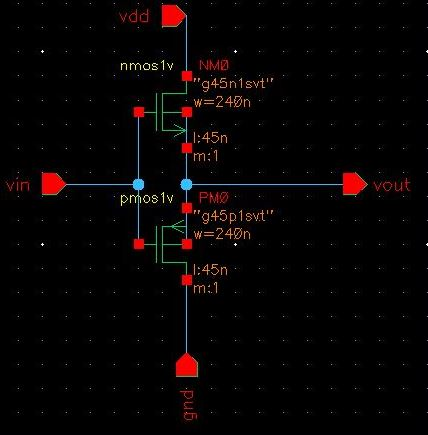
\includegraphics[scale=0.8]{../images/q2d_schematic.JPG}}
    \caption{Schematic of the Buffer circuit}
\end {figure}
The plot is simulated using a $V_{DD}$ value of 6V. Below is VTC plot of the buffer circuit.
\begin{figure} [H]
    \centering
    \makebox[\textwidth]{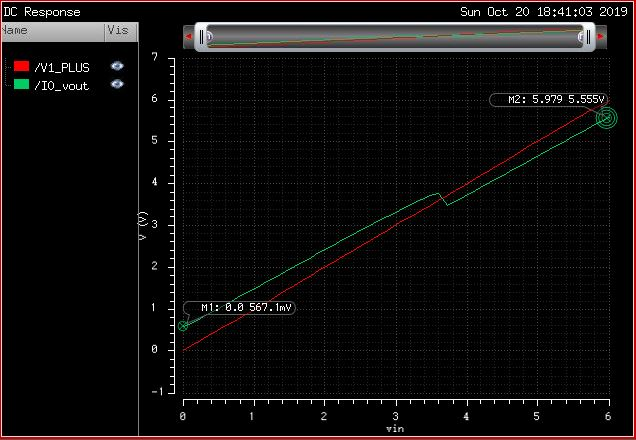
\includegraphics[scale=0.8]{../images/q2d_vtc.JPG}}
    \caption{The simulated VTC of the circuit}
\end {figure}
We can see from the endpoints of the green line, the $V_{out}$ plot that the output will always be between the bound of
$V_T$ (about 0.5V in this case), and $V_{DD} - V_T$ (about 5.5 in this case). The hystersis effect was not as exaggerated
as I had thought, and this is probably because I forgot to take into account that the overall deviation from an ideal buffer,
isn't that great.
\pagebreak



\section{Finding the Threshold Voltage and Body Bias of an NMOS Transistor}
\subsection{Finding the Body Bias $\gamma$}
Using the circuit defined in the problem, we can use the basic properties of the $V_{DS}$ vs $I_{D}$ curve to find the threshold voltage
for any $V_{SB}$. First we make the schematic for an NMOS in Cadence.
\begin{figure} [H]
    \centering
    \makebox[\textwidth]{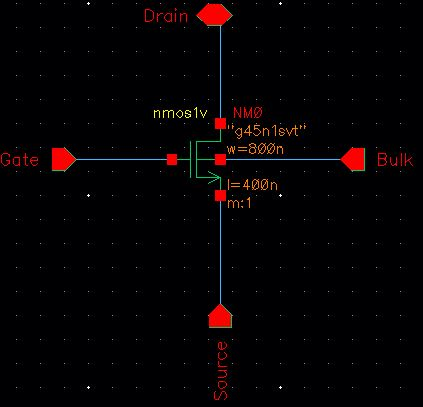
\includegraphics[scale=0.6]{../images/q3_400nm_schematic.jpg}}
    \caption{Schematic for L = 400nm NMOS}
\end{figure}
Then we can make the symbol for the nmos and connect sources and ground just like defined in the problem.
\begin{figure} [H]
    \centering
    \makebox[\textwidth]{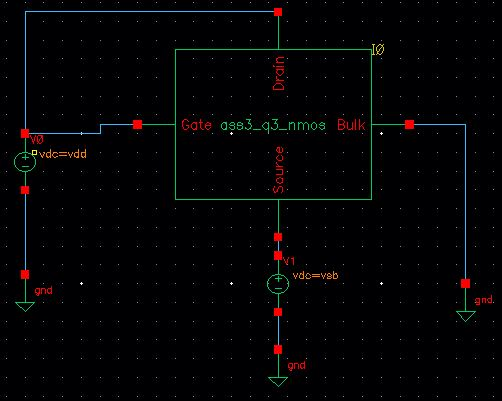
\includegraphics[scale=0.6]{../images/q3_400nm_tb_schematic.jpg}}
    \caption{Circuit for L = 400nm NMOS}
\end{figure}
We can sweep the gate and drain connected source at any $V_{SB}$ to obtain the the $V_{DS}$ vs $I_{D}$ plot and get the threshold voltage. For the case of 
L = 400nm and $V_{SB}$ = 0, the plot is shown below. The source voltage is swept from 0 to 5V.
\begin{figure} [H]
    \centering
    \makebox[\textwidth]{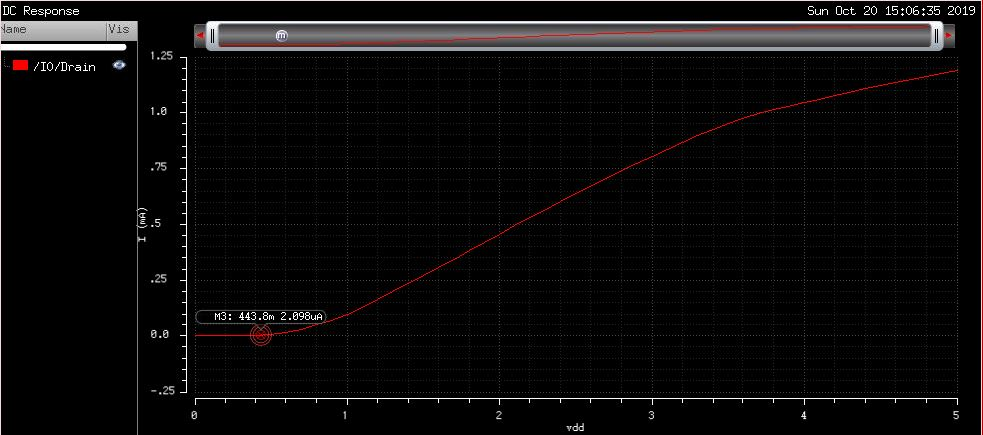
\includegraphics[scale=0.5]{../images/q3_400nm_vt0.jpg}}
    \caption{$V_{DS}$ vs $I_{D}$ plot for L = 400nm NMOS at $V_{SB}$ = 0}
\end{figure}
The vdd value at which the current begins to rise is taken as the threshold voltage. Here, because $V_{SB}$ = 0, the vdd value of 443.8mV is $V_{T0}$. For 
values where $V_{SB}$ is not equal to zero we must obtain $V_{GS} = V_{TN} = V_G - V_{SB}$ in order to perform correct calculations.
The method used to find values of $V_{TN}$ will only be visually shown once to prevent cluttering in the report. 

Once enough data points have been obtained, we apply the equation
\[V_{TN} = V_{T0} + \gamma (\sqrt{V_{SB} + |2\phi_F|} - \sqrt{|2\phi_F|}) \]
and substitute the obtained values, where $|2\phi_F|$ = 0.88V as defined in the question. The result is essentially a plot of a linear equation, with the independent
variable $\gamma$ being the slope. For this problem, I will be using 6 data points equally split between 0V $\leq V_{SB} \leq$ 1.8V.
\subsubsection{L = 400nm NMOS}
Using the method described above, we obtain the data points shown below. The values are in volts
\begin{table} [H]
    \centering
    \begin{tabular} {ccc}
        $V_{SB}$ & $V_{G}$ & $V_{TN} = V_{GS}$\\
        \hline
        0 & 0.4438 & 0.4438\\
        0.36 & 0.8560 & 0.4960\\
        0.72 & 1.2650 & 0.5450\\
        1.08 & 1.6550 & 0.5750\\
        1.44 & 2.0440 & 0.6000\\
        1.80 & 2.4190 & 0.6190\\
    \end{tabular}
    \caption{Voltages obtained from simulation for the L = 400nm NMOS}
\end{table}
Applying the respective values to the equation from before, we obtain the plot to get $\gamma$
\begin{figure} [H]
    \centering
    \makebox[\textwidth]{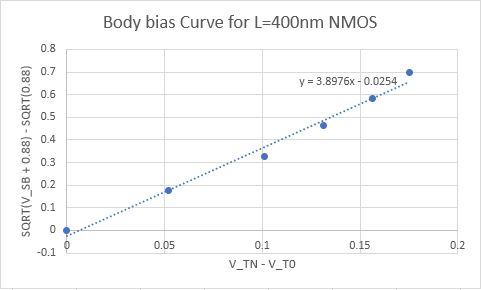
\includegraphics[scale=0.6]{../images/q3_400nm_gamma.jpg}}
    \caption{Body Bias plot for L=400nm Transistor}
\end{figure}
Taking the slope on the plot, get obtain $\gamma$ = 3.8976, and $V_{T0}$ = 0.4438.
\subsubsection{L = 100nm NMOS}
We now change the L of the NMOS to 100nm and apply the same method. The data points are shown in the table below, with values in volts.
\begin{table} [H]
    \centering
    \begin{tabular} {ccc}
        $V_{SB}$ & $V_{G}$ & $V_{TN} = V_{GS}$\\
        \hline
        0 & 0.4650 & 0.4650\\
        0.36 & 0.8792 & 0.5192\\
        0.72 & 1.3320 & 0.6120\\
        1.08 & 1.7280 & 0.6480\\
        1.44 & 2.1080 & 0.6680\\
        1.80 & 2.4580 & 0.6580\\
    \end{tabular}
    \caption{Voltages obtained from simulation for the L = 100nm NMOS}
\end{table}
Applying the respective values to the equation from before, we obtain the plot to get $\gamma$
\begin{figure} [H]
    \centering
    \makebox[\textwidth]{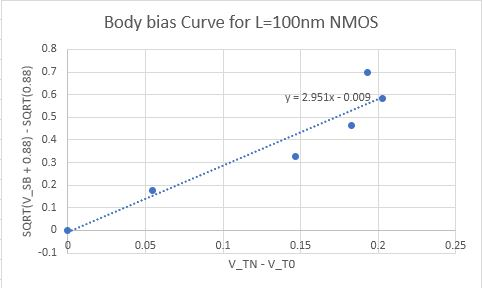
\includegraphics[scale=0.6]{../images/q3_100nm_gamma.jpg}}
    \caption{Body Bias plot for L=100nm Transistor}
\end{figure}
Taking the slope on the plot, get obtain $\gamma$ = 2.951, and $V_T0$ = 0.4650.

We can see that the reducing the value of L for the NMOS transistor creates a slight increase in the threshold voltage for the same
source-body bias values. Looking back at the current equations for a transistor, this makes sense as we saw that the current $I_d$ was 
inversely proportional to the term $L_n$. 
\subsubsection{Netlist}
The netlist for this problem is attached with the submission of the report, but for direct reading it is included here.

\rule{\textwidth}{1pt}
// Library name: ELEC402\\
// Cell name: ass3\_q3\\
// View name: schematic\\
subckt ass3\_q3 Bulk Drain Gate Source\\
    NM0 (Drain Gate Source Bulk) g45n1svt w=(800n) l=100n nf=1 as=112f \\
        ad=112f ps=1.88u pd=1.88u nrd=175m nrs=175m sa=140n sb=140n
        sd=160n sca=55.42636 scb=0.04134 scc=0.00529 m=(1)
ends ass3\_q3\\
// End of subcircuit definition.\\

// Library name: ELEC402\\
// Cell name: ass3\_q3\_tb2\\
// View name: schematic\\
I0 (0 V0\_PLUS V0\_PLUS V1\_PLUS) ass3\_q3\\
V1 (V1\_PLUS 0) vsource dc=vsb type=dc\\
V0 (V0\_PLUS 0) vsource dc=vdd type=dc\\
\rule{\textwidth}{0.5pt}
\subsection{Confirming the value of $|2\phi_F|$}
The value $\phi_F$ is a value that is dependent on the doping of the materials and the temperature. So, the value we are using for $2\phi_F$
is currently assuming the conditions of the material and the environment temperature. 

In the case where we are given other parameters of the transistor that define the body-effect coefficient $\gamma$, we could use the 
same method of obtaining $V_{GS}$, but for only a single $V_{SB}$.

\pagebreak

\section{Capacitance of a PMOS transistor}
\subsection{Computing gate capacitances}
The value $C_{ox}$ is used consistently, so it is computed first.
\[C_{ox} = \frac{\epsilon _{ox}}{t_{ox}} \]
We are taking the value $\epsilon _{ox}$ as the one shown in lecture $4.2*\epsilon _0$ for $SiO_2$, and $t_{ox}$ = 4nm. So,
\[C_{ox} = \frac{4.2*8.854*10^{-12}}{4*10^{-9}} \]
\[C_{ox} = 9.2967*10^{-3} Fm^{-1}\]
We also need to include overlap capacitance.
\[C_{ov} = C_{ox} * L_{diffusion} \]
\[C_{ov} = 9.2967*10^{-3} * 22 * 10^{-9} \]
\[C_{ov} = \SI{0.2045}{fF \mu m^{-1}}\]
\subsection*{Worst case gate capacitance}
The worst case gate capacitance also includes the overlap capacitances. It is given by 
\[C_g = C_{ox} * W * L + 2*C_{ov}\]
Because we want per unit width capacitance, we ignore the W term an only include L.
Substituting in,
\[C_g = 9.2967*10^{-3} * 180*10^{-9} + 2 * C_{ov}\]
\[C_g = \SI{2.0824}{fF \mu m^{-1}}\]
\subsection*{Calculating $C_{GS}$, $C_{GD}$ and $C_{GB}$}
So, to calculated the 3 quantities, we use the equations, shown in the table below. 
\begin{table} [H]
    \centering
    \begin{tabular} {c|ccc}
        & Cutoff & Linear & Saturation \\
        \hline
        $C_{GS}$& 0 & $\frac{1}{2}C_{ox}WL + C_{ov}$ & $\frac{2}{3}C_{ox}WL + C_{ov}$ \\
        $C_{GD}$& 0 & $\frac{1}{2}C_{ox}WL + C_{ov}$ & 0\\
        $C_{GB}$& $C_{ox}WL$ & 0 & 0\\
    \end{tabular}
    \caption{Equations used to calculate capacitances}
\end{table}
Substituting the repsective values yields the table below, where all values are in fF.
\begin{table} [H]
    \centering
    \begin{tabular} {c|ccc}
        & Cutoff & Linear & Saturation \\
        \hline
        $C_{GS}$& 0 & 2.8354 & 3.08644 \\
        $C_{GD}$& 0 & 2.8354 & 0\\
        $C_{GB}$& 1.5061 & 0 & 0\\
    \end{tabular}
    \caption{Calculated capacitances for PMOS}
\end{table}
\subsection{Computing worst case capacitance}
To compute worst case capacitance $C_j$ we need to first find base junction capacitance $C_{jb}$ and the built in potential
$\phi _B$. First we find $\phi _B$ using the values given, and the $n_i$ value used in the lectures in the equation
\[\phi_B = \frac{kT}{q}\ln{\frac{N_A N_D}{{n_i}^2}} \]
Substituting and solving yields
\[\phi_B = \SI{0.9358}{V}\]
For $C_{jb}$ we use the equation
\[C_{jb} = \sqrt{ \frac{\epsilon_{Si}q}{2\phi_B} \frac{N_A N_D}{{n_i}^2}    }\]
Substituting and solving yields
\[C_{jb} = \SI{0.5151}{fF \mu m^{-2}} \]
The general equation to solve for the drain junction capacitance is 
\[C_j = \frac{C_{jb} * (Y + x_j) * W}{ (1 - \frac{V_j}{\phi_B})^m      } \]
where $V_j$ is the base-drain junction voltage and m = 0.5. If we assume the n-well is a rectangular prism, 
the worst case takes into account the side edges of the the well. The worst case junction voltage would be 0V.
\[C_j = C_{jb} * ((Y + x_j) * W + 2 * W * x_j) \]
Substituting known values yields
\[C_{j_{worstcase}} = \SI{0.78804}{fF}\]
\subsection{Computing drain junction capacitance}
\subsubsection{$V_D$ = 1.8V, $V_B$ = 0V}
Here $V_j$ = -1.8V. Substituting the known values into the previous general equation yields
\[C_j = \SI{0.2982}{fF}\]
\subsubsection{$V_D$ = 0V, $V_B$ = 0V}
Here $V_j$ = 0V. Substituting the known values into the previous general equation yields
\[C_j = \SI{0.5099}{fF}\]
\pagebreak

\section{Calcaulting Vs of 2-input NOR gates}
The first thing to do is to get the circuit for the NOR gate at the transistor level. We use the method taught in class
\begin{enumerate}
    \item Take the dual of the original function: $F = \overline{A + B}$ becomes $F = \overline{\overline{A + B}} = A + B$.
    \item Create the NMOS pull-down network: $A + B$ means parallel NMOS.
    \item Create the PMOS pull-up network: parallel NMOS means series PMOS.
    \item Combine the two networks: The result is the circuit shown below.
\end{enumerate}
\begin{figure} [H]
    \centering
    \makebox[\textwidth]{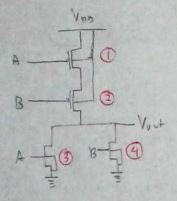
\includegraphics[scale=1]{../images/q5_nor.jpg}}
    \caption{Circuit for a 2-input NOR gate}
\end{figure}
\subsection{Theoretical calculations}
For the theoretical calculations, we first need to define the values we are using for calculations (some will also be used for simulation).
\begin{itemize}
    \item $V_{DD}$ = 1.8 V, becuase for simulation, we are using the GPDK45 specs.
    \item $V_{TN}$ = $|V_{TP}|$ = 0.4V, assuming they are the same type, where values are taken from Useful\_Formula.pdf on Canvas.
    \item $L_N$ = $L_P$, which will cancel out in calculations.
    \item $E_{CN}$ = $\SI{6}{V \mu m^{-1}}$ and $E_{CP}$ = $\SI{24}{V \mu m^{-1}}$, which are are taken from Useful\_Formula.pdf on Canvas, but will also notably cancel out.
    \item $W_N$ = $6\lambda$ = $\SI{135}{nm}$ and $W_P$ = $24\lambda$ = $\SI{675}{nm}$ , which are defined by the problem and the fact we are using 45nm technology.
\end{itemize}
For referencing of the transistors in the calculations, each transistor has been numbered in the circuit drawing.
\subsubsection{One input switching}
For the case of one input switching, we take the input A to be logic 0 and the input B to be the one that switches. To get the value of $V_S$
we simply need to equate currents at the $V_{out}$ node. Because we are calculating for $V_S$, the conditions for this calcultion are therefore
\[V_{B} = V_{out} = V_S \quad and \quad  V_A = 0\]
We notice that PMOS1 and PMOS2 are operating in the saturation, and NMOS4 is also operating in saturation. NMOS3 is operating in the cut-off region.
The the currents that matter for this case are the drain currents of PMOS2 and NMOS4.
\[I_{D-nmos4}(saturation) = I_{p-nmos2}(saturation) \]
Using the same equations used in section 1, cancelling identical terms and approximating yields the equation
\[2\chi^2(V_S - V_{TN})^2 = (V_{DD} - 2V_{TP} - V_S)^2 \quad\quad where \quad \chi = \sqrt{\frac{\frac{ W_N }{E_{CN}L_N  }}{\frac{ W_P }{E_{CP}L_P  }}} \]
Now we can solve for $V_S$
\[V_S = \frac{ V_{DD} + V_{TN}\chi - 2*V_{TP}  }{\chi + 1} \]
Substituting the values from before yields the value of $V_S$
\[V_S = \SI{0.7167}{V} \]
\subsubsection{Two inputs tied together}
For the case of two inputs being tied together, we take similar conditions to the previous case, except now the input A is also equal to $V_S$
\[V_A = V_{B} = V_{out} = V_S\]
Thus PMOS2, NMOS3 and NOMS4 are operating in saturation and PMOS1 is operating in the linear regime. The currents that matter for this case are the 
drain currents of PMOS4 and the sum of the drain currents of NMOS3 and NMOS4.
\[I_{D-nmos4}(saturation)+I_{D-nmos3}(saturation)= I_{p-nmos2}(saturation) \]
Because the NMOS transistors are the same we can just take 2 drain currents of the NMOS
\[2*I_{D-nmos}(saturation)= I_{p-nmos2}(saturation) \]
Using the same equations used in section 1, cancelling identical terms and approximating yields the equations
\[2\chi^2(V_S - V_{TN})^2 = (\frac{V_{DD} - 3*V_S}{2} - V_{TP})^2 \quad\quad where \quad \chi = \sqrt{\frac{\frac{ W_N }{E_{CN}L_N  }}{\frac{ W_P }{E_{CP}L_P  }}} \]
Now we can solve for $V_S$
\[V_S = \frac{ V_{DD} + V_{TN}\chi*2\sqrt{2} - 2*V_{TP}}{2\sqrt{2}\chi + 3} \]
Substituting the values from before yields the value of $V_S$
\[V_S = \SI{0.36381}{V} \]
\subsection{Simulation Results}
Below is the schematic made for the NOR gate.
\begin{figure} [H]
    \centering
    \makebox[\textwidth]{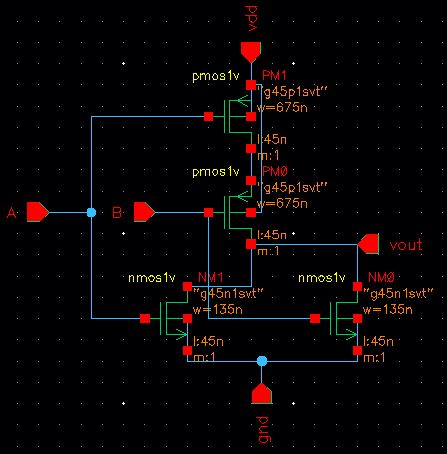
\includegraphics[scale=0.65]{../images/q5_schematic_nor.jpg}}
    \caption{Schematic for the NOR gate}
\end{figure}
\subsubsection{One input switching}
Below is the testbench schematic made for the NOR gate with only one input switching.
\begin{figure} [H]
    \centering
    \makebox[\textwidth]{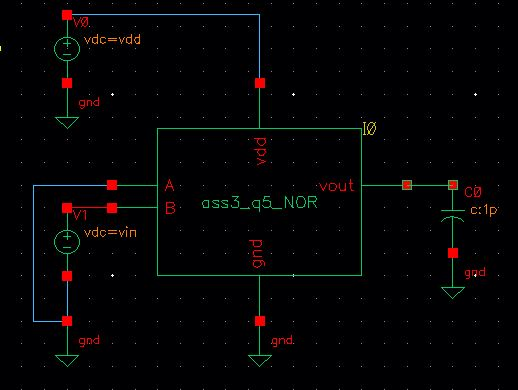
\includegraphics[scale=0.65]{../images/q5_tb_schematic_one.jpg}}
    \caption{Testbench schematic for the one input switching NOR gate}
\end{figure}
We can obtain $V_S$ by simulating the VTC of the testbench circuit. The result is shown below.
\begin{figure} [H]
    \centering
    \makebox[\textwidth]{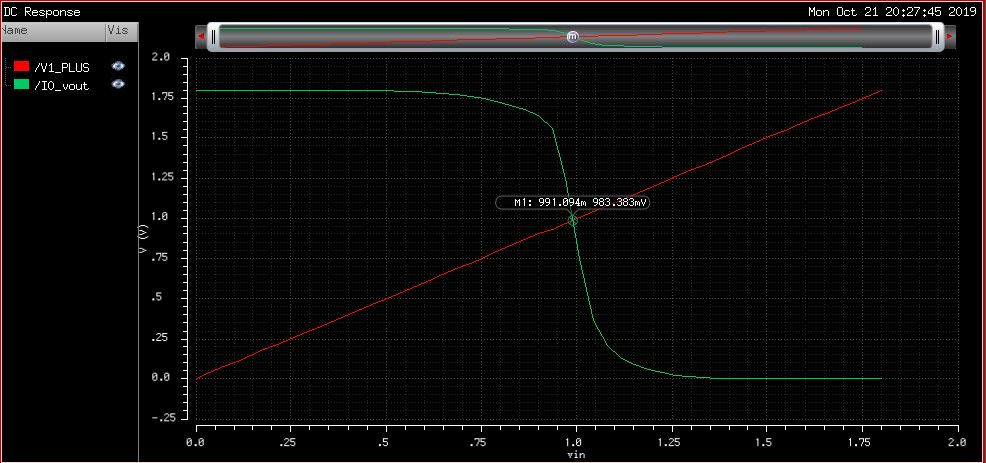
\includegraphics[scale=0.65]{../images/q5_tb_vtc_one.jpg}}
    \caption{VTC of the one input switching NOR gate}
\end{figure}
From the plot we can see that $V_S$ is simulated to be at a value of approximately $\SI{1}{V}$.
\subsubsection{Two inputs tied together}
Below is the testbench schematic made for the NOR gate with only both inputs switching.
\begin{figure} [H]
    \centering
    \makebox[\textwidth]{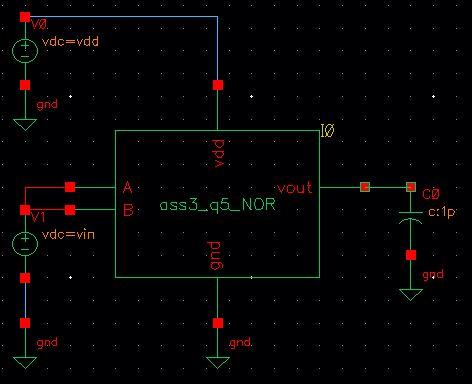
\includegraphics[scale=0.65]{../images/q5_tb_schematic_both.jpg}}
    \caption{Testbench schematic for the one input switching NOR gate}
\end{figure}
We can obtain $V_S$ by simulating the VTC of the testbench circuit. The result is shown below.
\begin{figure} [H]
    \centering
    \makebox[\textwidth]{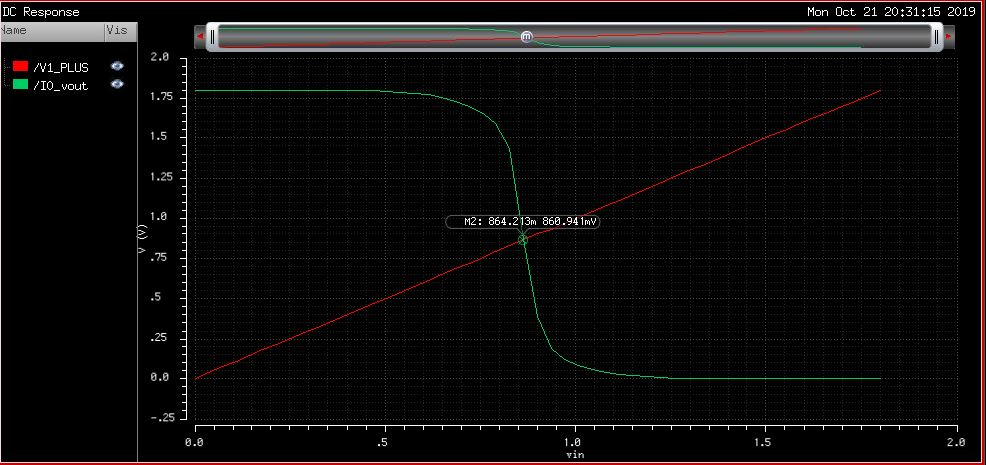
\includegraphics[scale=0.65]{../images/q5_tb_vtc_both.jpg}}
    \caption{VTC of the one input switching NOR gate}
\end{figure}
From the plot we can see that $V_S$ is simulated to be at a value of approximately $\SI{0.861}{V}$.
\subsubsection{Explaining the Discrepancy between theory and simulation}
Based on the simulations, we can see that the theoretical value is off the simulated value by approximately 30-40 percent. There are two main sources
of error: the calculation values (such as $V_TN$ and $V_TP$) and approximations done in the calculations.

For the calculation values, we used values that were defined separately from this assignment, so they would not be exactly the same as the actual 
specifications of the transistor. If we look at the threshold values, we saw in Section/Problem 3 threshold voltage values that were not the used value of
$\SI{0.4}{V}$, rather somewhat higher. This value plays a large role in the equations derived for $V_S$ and thus may have affected the 'real' value of 
$V_S$.

The approximations made in the derivation of the equation for the switching voltage also may have impacted the 'real' value of $V_S$, although not by
much.
\pagebreak

\section{Noise Margins of a Saturated-enhancement load inverter}
Below is a schematic of the circuit itself. Because the GPDK package is defined for 45nm technology, the lowest possible length is 120nm.
So instead of 1$\mu$m and 100nm lengths, I am using 120nm and 1.2$\mu$m. Below is the schematic for the circuit.
\begin{figure} [H]
    \centering
    \makebox[\textwidth]{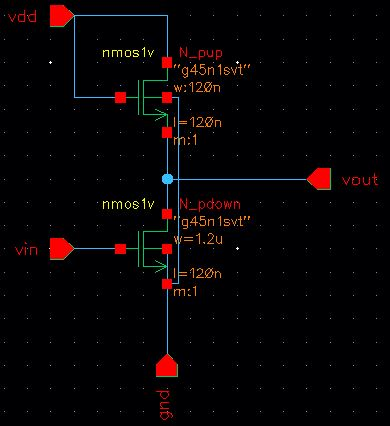
\includegraphics[scale=0.65]{../images/q6_schematic.jpg}}
    \caption{Schematic for the saturated-enhancment load inverter}
\end{figure}
For the testbench, the typical components vpulse, vdc, and cap are used. The value of the capcitors were
specially chosen to be $\SI{2}{fF \mu m^{-1}}$. The pulse source, vpulse, is set to alternate between values of 0 and $V_{DD}$, and its 
rise, fall and period are defined the same was as shown in the tutorial.
The testbench schematic is shown below
\begin{figure} [H]
    \centering
    \makebox[\textwidth]{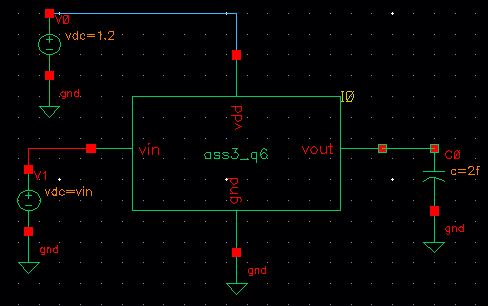
\includegraphics[scale=0.85]{../images/q6_tb_schematic.jpg}}
    \caption{Testbench schematic for the saturated-enhancment load inverter}
\end{figure}
\pagebreak
Running the simulation, the resulting waveform is shown below.
\begin{figure} [H]
    \centering
    \makebox[\textwidth]{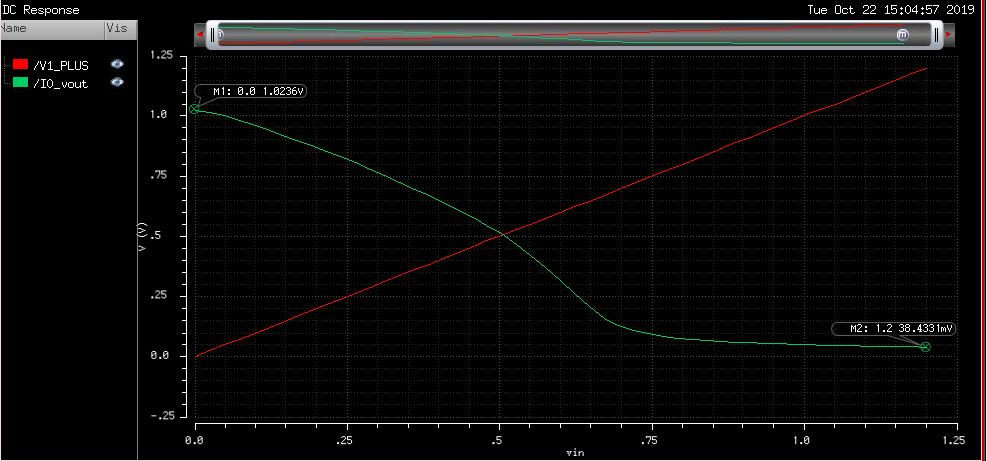
\includegraphics[scale=0.6]{../images/q6_tb_waveform.jpg}}
    \caption{Simulation of the saturated-enhancement load inverter}
\end{figure}
The values important for calculating noise margin are $V_{IL}$, $V_{IH}$, $V_{OL}$ and $V_{OH}$, and are noted by the selected points in the waveform.
The values are not too clear in the image, so for clarity they are shown in the table below, with units in volts.
\begin{table} [H]
    \centering
    \begin{tabular} {cccc} 
        $V_{IL}$ & $V_{IH}$ & $V_{OL}$ & $V_{OH}$\\
        \hline
        0 & 1.2 & 0.023568 & 0.6639
    \end{tabular}
    \caption{Noise margin voltages from the waveform}
\end{table}
We use the following equations to calcaulte for noise margins.
\[NM_L = V_{IL} - V_{OL} \quad and \quad NM_H = V_{OH} - V_{IH}\]
Substituting the values in the table above will yield the noise margin values
\[NM_L = \SI{-23.5681}{mV} \quad and \quad NM_H = \SI{-536.08}{mV}\]
We can attribute the large high noise margin $NM_H$ due to the large width of the pull-down NMOS transistor ($10*L$). As we learned in class, the 
saturated-enhancement load inverter is a ratioed inverter, meaning the performance of the inverter is dependent on a ratio of specifications.
For this inverter, this ratio is dependent on the gate widths and lengths of both transistors.



\end{document}